\documentclass[11pt,titlepage]{article}
\usepackage{pset}

\newcommand*{\X}{\mathfrak{X}}
\newcommand*{\Mod}{\mathcal{M}}
\newcommand*{\vbar}{\;\big\vert\;}
\DeclareMathOperator{\Mixt}{Mixt}
\DeclareMathOperator{\Sec}{Sec}
\DeclareMathOperator*{\argmax}{arg\ max}

\title{The Restricted Boltzmann Machine}
\author{Aaron Pribadi}
\date{November 2011}

\begin{document}

\maketitle

\tableofcontents

\pagebreak

\section{What is Algebraic Statistics?}

    Algebraic statistics is a relatively new field that examines statistical
    problems using algebraic geometry and commutative algebra.  One advantage of
    this approach is the availability of computational tools once a problem has
    been cast in the language of algebra.  For example, Gröbner bases and
    related techniques have been used in Monte Carlo algorithms to sample from
    probability distributions.  The analysis of contingincy tables by this
    method in \cite{DS98} provided one of the first connections between
    commutative algebra and statistics.

    Algebraic statistics also provides a geometric view of the central objects
    of statistics, e.g. probability distributions and families of probability
    distributions.  By `geometric' we mean that we rely upon intrinsically
    defined objects in lieu of particular explicit coordinatizations.  In this
    light, algebraic statistics might be seen as in the tradition of
    \emph{information geometry}, a field pioneered in the 1980s that applied the
    techniques of Riemannian geometry to probability models.

    An introduction to the field of algebraic statistics may be found in
    \cite{DSS09} and a brief history of the field may be found in \cite{Ricc09}.


\section{Probability Models}
    \subsection{The Probability Simplex}
    For simplicity, the probability distributions that we consider are
    distributions over finite sets.  The corresponding geometric object, the
    simplex, is relatively straightforward.  
    
    \begin{definition} The \emph{probability simplex} of dimension $n$ (also
    called the \emph{standard simplex}) is the space
    \[
        \Delta_{n} = 
        \left\{(x_0, \ldots, x_{n}) \vbar \sum_{i=0}^{n} x_i= 1, x_i \ge 0 \right\} 
        \cong 
        \left\{(x_1, \ldots, x_{n}) \vbar \sum_{i=1}^{n} x_i \le 1, x_i
        \ge 0 \right\}.
    \]
    \end{definition}
    A simplex in general is the image of a standard simplex under any affine
    transformation.  Low dimensional simplices are familiar objects; $\Delta_0$
    is a point, $\Delta_1$ is a line segment, $\Delta_2$ is a triangle,
    and $\Delta_3$ is a tetrahedron.
    \begin{center}
    \scalebox{1}{ 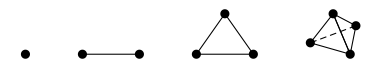
\includegraphics[scale=0.5]{images/simplices.png} }
    \end{center}
    A simplex is the locus of a finite collection of polynomial equations and
    polynomial inequalities and therefore is a semialgebraic set.

    A point in the simplex $\Delta_{n-1}$ corresponds to a probability
    distribution over $n$ states in the natural way; each coordinate $x_i$
    corresponds to the probability $p(i)$ of the event $i$ occuring.  By the
    phrase \emph{statistical model}, we mean a subset $\Mod \subset \Delta_n$
    corresponding to a family of probability distributions.  In the context of
    algebraic statistics, we usually look at statistical models that are
    semialgebraic sets.

\subsection{The Independence Model}
    Independence conditions arise naturally in many statistical questions.
    Essentially, they allow portitions of a model to be considered separately.

    First, we introduce some notation.  For any positive integer $m$, let $[m] =
    \{1, 2, \ldots, m\}$; this is used when we need a finite set with $m$
    elements.

    Suppose that the random variables $X$ and $Y$ have state spaces $[r]$ and
    $[c]$, respectively.  By definition, $X$ and $Y$ are independent if their
    joint distribution over $[r] \times [c]$ factors into a distribution over
    $[m]$ and another over $[n]$.  
    
    Then the independence model $\Mod \subset \Delta_{rc - 1}$ is the space of
    distributions of the form
    \[
        P(X = i, Y = j) = p_i q_j
        \qquad
        \text{where $p \in \Delta_{m-1}$ and $q \in \Delta_{n-1}$}.
    \]
    \begin{example}
    If $r = c = 2$ (i.e. if $X$ and $Y$ are binary) then the possible
    distributions look like
    \begin{center}
    \begin{tabular}{l|cc}
    & $X = 1$ & $X = 2$\\
    \hline
    $Y = 1$ & $\alpha\beta$ & $(1-\alpha)\beta$\\
    $Y = 2$ & $\alpha(1-\beta)$ & $(1-\alpha)(1-\beta)$
    \end{tabular}
    \end{center}
    for some $\alpha, \beta \in [0,1]$.  
    \end{example}

    Another way to view the independence model is as the set of all $r\times c$
    matrices of rank 1 with non-negative entries that sum to 1.  For a matrix of
    rank 1, all rows (and columns) are multiples of each other, so the rank 1
    condition is equivalent to the condition that the distribution factors.
    
    The independence model has the parametrization
    \begin{IEEEeqnarray*}{rCrCl}
        \phi &:& \Delta_{m-1} \times \Delta_{n-1} &\to& \Mod \subset \Delta_{rc-1}\\
        && \phi_{ij}(p, q) &=& p_i q_j.
    \end{IEEEeqnarray*}
    The model $\Mod$ also has an implicit description.  The points in the variety
    \[
        V = \cdil[\big]{
        \phi \in \R^{rc} 
        \vbar
        \phi_{ij} - (\phi_{i+})(\phi_{+j}) = 0
        \quad
        \text{for all $i \in [m]$ and $j \in [n]$}
        }
    \]
    satisfy the independence condition because the probability $\phi_{ij}$ that
    $(i,j)$ occurs must factor into the probability $\phi_{i+}$ that $i$ occurs
    and the probability $\phi_{+j}$ that $j$ occurs.  The independence model is
    then the intersection $\Mod = V \cap \Delta_{rc-1}$, and is clearly a
    semialgebraic set.

\subsection{Hidden Variables and Mixture Models}
    Consider a random variable $X$ with state space $[r]$, and suppose that
    another random variable $Y$ with state space $[c]$ has an influence on $X$.
    If $Y$ has some prior distribution $\pi$, then the joint distribution of $X$
    and $Y$ is 
    \[
        P(X = i, Y = j) = \pi_j \cdot p_i^{(j)}
    \]
    where $\{p^{(j)} \mid j \in [c]\}$ is some collection of distributions.

    If $Y$ is a hidden variable, we can only observe the marginal distribution
    of $X$.  The marginal probability is the sum over the possible hidden values
    \[
        P(X = i) = \sum_{j \in [c]} \pi_j \cdot p_i^{(j)}.
    \]
    A hidden variable model allows for the creation of a potentially more
    complex model out of simple components $p^{(j)} \in \Delta_{r-1}$.
    In particular, if the distributions $p^{(j)}$ are required to lie in some
    model $V \subset \Delta_{r-1}$, then we have a mixture model.
    \begin{definition}
    Suppose that $V$ and $W$ are subsets of the affine space $\R^n$.  Their
    \emph{mixture} is the set
    \[
        \Mixt(V, W) = \cdil[\big]{
        \lambda v + (1 - \lambda)w \vbar
        v \in V, w \in W, \lambda \in [0,1]
        }.
    \]
    A mixture of $V$ with itself $k$ times produces the higher mixture
    \[
        \Mixt^k(V) = \cdil*{
        \sum_{i=1}^k \lambda_i v_i \vbar v_i \in V, \lambda_i \in [0,1],
        \text{and }\lambda_1 + \cdots \lambda_s = 1
        }.
    \]
    A \emph{mixture model} is a statistical model produced by mixtures.
    \end{definition}

    \begin{example}
    A \emph{Gaussian mixture model} is a simple model that is useful in a wide
    variety of situations.  A Gaussian distribution with parameters $(\mu,
    \sigma)$ has probability density
    \[
        p_{\mu, \sigma}(x) = \frac{1}{\sqrt{2\pi\sigma^2}} 
        \exp\pdil*{-\frac{(x - \mu)^2}{2\sigma^2}}.
    \]
    A mixture of two Gaussian distributions is a weighted sum $p(x) = \lambda
    p_{\mu_1, \sigma_1}(x) + (1 - \lambda)p_{\mu_2, \sigma_2}(x)$.  
    \begin{center}
    \scalebox{1}{ 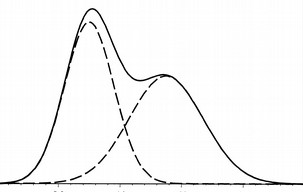
\includegraphics[scale=0.5]{images/mixture.png} }
    \end{center}
    (The space of distributions over the real line is not finite dimensional,
    but in this case works similarly.) Mixtures of more or higher dimensional
    Gaussian distriubtions are defined as one would expect.  Such models are
    useful, for instance, for clustering tasks.
    \end{example}

    Mixture models correspond to a relatively well-studied object in algebraic
    geometry.
    \begin{definition}
    The \emph{secant variety} of the affine variety $V \subset \F^n$ is
    \[
        \Sec(V) = \overline{\cdil[\big]{
        \lambda u + (1 - \lambda) v \vbar
        u,v \in V
        \text{ and }
        \lambda \in \F
        }}
    \]
    where the line indicates the Zariski closure of the set.  Higher secant
    varieties are defined in the natural way, that is, $\Sec^1(V) = V$ and
    $\Sec^k(V) = \Sec(Sec^{k-1}(V), V)$ for $k \ge 2$.
    \end{definition}

    There is a reasonably straightforward relationship between mixture models
    and secant varieties.
    \begin{proposition}[\cite{DSS09}]
    If $V$ is a semialgebraic set, then the secant variety
    $\Sec^k(\overline{V})$ is the Zariski closure of the mixture $\Mixt^k(V)$.
    \end{proposition}

\subsection{Graphical models}

    A graphical model is a probabilistic model for which a graph (directed or
    undirected) represents the conditional independence structure between random
    variables. 

    Let $G$ be a graph with vertex set $V$.  Suppose that $(X_\alpha)_{\alpha
    \in V}$ are random variables.  It is common for the $X_\alpha$ to be either
    discrete or real-valued.  The joint probability of $X = (X_\alpha)$ is said
    to factor with respect to $G$ if the probability density is
    \[
        p(X_1, \ldots, X_n) = 
            \prod_\alpha p(X_\alpha \mid X_\beta, \beta \text{ is a parent of }
            \alpha).
    \]
    The dependence of a random variable on the other variables is completely
    captured by its dependence on its immediate parents (i.e. on the variables
    having directed edges into it).  It is also possible to formulate an
    equivalent statement in terms of conditional independence statements.

    In the case of an undirected graph, it is known (in a result called the
    Hammersley–Clifford theorem) that the probability density factors as
    \[
        p(X_1, \ldots, X_n) = 
            \prod_{S \in C(G)} p(X_\alpha \mid X_\beta, \beta \in S)
    \]
    where the $S$ are complete subgraphs (cliques) of $G$.

    Graphical models turn up in a number of places: Bayesian networks (directed)
    and Markov random fields (undirected) in statistics, Boltzmann machines in
    machine learning, and Ising models (particle spins in a lattice) in
    statistical mechanics.

\subsection{Maximum Likelihood}

    One way to select a particular probability distribution $p$ from a model
    $\Mod$ is by \emph{maximum likelihood}.  That is, given observations
    $X^{(1)}, \ldots, X^{(N)}$ we attempt to find the distribution $p \in \Mod$
    that maximizes the likelihood
    \[
        L(p \mid X^{(1)}, \ldots, X^{(N)}) = \prod_{i=1}^N p(X^{(i)}).
    \]
    The log-likelihood $l(p \mid X^{(i)}) = \log\pdil[\big]{L(p \mid X^{(i)})}$
    is sometimes used in place of the likelihood.

    Given a parametrized model $\Mod = \{p_\theta \mid \theta \in \Theta\}$, the
    parameter 
    \[
        \hat\theta = \argmax_{\theta \in \Theta} l(p_\theta \mid X^{(i)})
    \]
    that maximizes the likelihood is referred to as the \emph{maximum-likelihood
    estimator}.  For most models, the maximum likelihood satisfies a number of
    asymptotic optimality conditions.


\section{The Restricted Boltzmann Machine}

\subsection{An Introduction}
    We will now focus on a statistical model that has recently become important
    to the machine learning community; it is the building block for a number of
    new techniques.
    \begin{definition}
    The \emph{Restricted Boltzmann Machine} (RBM) with $n$ visible variables and
    $k$ hidden variables is a model with states of the form $(v, h)$ where $v
    \in \{0,1\}^n$ and $h \in \{0,1\}^k$.  It is parametrized by a real $k
    \times n$ matrix $W$ and vectors $b \in \R^n$, $c \in \R^k$, so that it has
    a total of $nk + n + k$ real parameters.  Its unnormalized joint
    distribution is
    \[
        \psi(v, h) = \exp(h^T W v + b^Tv + c^T h)
    \]
    and its actual joint distribution is 
    \[
        p(v, h) = \frac{\psi(v,h)}{Z}
    \] 
    where the normalizing constant $Z = \sum_{v,h} \psi(v, h)$ is the called the
    \emph{partition function}.  
    \end{definition}

    The `energy' of the system $H = h^T W v + b ^T v + c^T h$ is a quadratic
    polynomial in the visible and hidden variables.  A general (as opposed to
    restricted) Boltzmann machine would allow cross-terms between all variable
    pairs.

    Because interactions between variables are restricted to those between a
    visible and a hidden variable, the RBM factors with respect to the complete
    bipartite graph $K_{n,k}$.
    \begin{center}
    \scalebox{1.0}{ 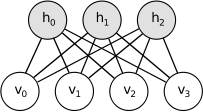
\includegraphics[scale=0.8]{images/rbm.png} }
    \end{center}
    Notice that the terms in $H$ become multiplicative factors when
    exponentiated.  Thus terms that only involve some subset of the variables
    correspond to multiplicative factors that only involve those variables; from
    this we can derive the appropriate independence conditions. 
    
    The marginal distribution of the RBM over its visible variables is
    \[
        p_V(v) = \sum_{h \in \{0,1\}^k} p(v, h).
    \]
    Given a fixed value $h$ for the hidden variables, the visible variables are
    all independent.  It follows that the marginal distribution over the visible
    variables is a mixture of independence models.  The mixture model can have
    up to $2^k$ components, because there are $2^k$ possible states for the
    hidden variables.

    In some sense, the hidden variables constitute an `explanation' for the
    observed variables.  That is, a particular value of $v$ induces a
    probability distribution over possible values $h$ of the hidden variables.
    This observation motivates a number of uses for the RBM, including as the
    building block for the Deep Belief Network, discussed later.

\subsection{The Geometry of the RBM}
    The recent paper \cite{CMS09} examines the RBM from an algebro-geometric
    perspective.
    
    In the framework of algebraic geometry, we want a polynomial parametrization
    of the RBM.  To that aim, use the parametrization
    \[
        \gamma_i = \exp(c_i)
        \qquad
        \omega_{ij} = \exp(W_{ij})
        \qquad
        \beta_j = \exp(b_j)
    \]
    as $\gamma_i$, $\omega_{ij}$, and $\beta_j$ range over strictly positive
    real values.  Under this parametrization, the unnormalized probability
    distribution is
    \[
        \psi(v, h) = \prod_{i=1}^k \gamma_i^{h_i}
            \cdot 
            \prod_{i=1}^k \prod_{j=1}^n \omega_{ij}^{h_i v_j}
            \cdot
            \prod_{j=1}^n \beta_j^{v_j},
    \]
    and therefore is given by polynomials (monomials, even).  The partition
    function $Z$ is also a polynomial in the new parameters.  Thus the full
    parametrization $\R_{>0}^{nk+n+k} \to \Delta_{2^n-1}$ of the model is a
    polynomial map.  The image $M_n^k \subset \Delta_{2^n - 1}$ of the map is a
    semialgebraic set.  The marginalized probabilities for the visible variables
    factor as
    \[
        p_V(v) = \frac 1 Z
        \beta_1^{v_1} \beta_2^{v_2} \cdots \beta_n^{v_n} 
        \prod_{i=1}^k(1 +
        \gamma_i 
        \omega_{i1}^{v_1}
        \omega_{i2}^{v_2}
        \cdots
        \omega_{in}^{v_n}
        )
    \]
    (the product over $i$ may be thought of as a generating function over
    the possible hidden values).

    In addition to the semialgebraic set $M_n^k \subset \Delta_{2^n - 1}$, we
    may also consider the corresponding projective variety.  There is a natural
    embedding of $\Delta_{2^n-1}$ into the real projective space
    $\Proj_\R^{2^n-1}$ and from there to the complex projective space
    $\Proj^{2^n-1}$.  Let $V_n^k \subset \Proj^{2^n-1}$ be the is the Zariski
    closure of $M_n^k$ in complex projective space.

    In the absence of `problems', one would expect that both $M_n^k$ and $V_n^k$
    have the same dimension as the parameter space $\R^{nk + n + k}$.  In fact,
    the dimensions are
    \[
        \dim M_n^k = \dim V_n^k = \min\{nk+n+k, 2^n -1\}
    \]
    when $k \le 2^{n - \lceil \log_2(n+1) \rceil}$, which includes most cases of
    practical interest.

    The paper \cite{CMS09} also shows that the varieties $M_n^k$ and $V_n^k$
    `factor'.  Specifically, they factor as \emph{Hadamard powers}
    \[
        V_n^k = (V_n^1)^{[k]}
        \qquad
        M_n^k = (M_n^1)^{[k]}.
    \]
    Then $M_n^1$ and $V_n^1$ are examined.  The variety $V_n^1$ conincides with
    the first secant variety of the \emph{Segre embedding} of the product of
    projective lines $(\Proj^1)^n$ into $\Proj^{2^n-1}$.  The corresponding
    statistical model $M_n^1$ with one hidden value is a mixture of two
    independence models.

    Both the Hadamard product and the Segre embedding are standard
    algebro-geometric constructions.  The Hadamard product $X * Y$ of two
    subvarieties $X$ and $Y$ of a projective space $\Proj^n$ is defined to be
    the Zariski closure of the image of the rational map
    \[
        X \times Y \dashrightarrow \Proj^m,
        \quad
        (x, y) \mapsto [x_0y_0: x_1y_1 : \cdots : x_n y_n].
    \]
    The Segre embedding of the cartesian product of two subvarieties $X \subset
    \Proj^m$ and $Y \subset \Proj^n$ is the image of the map
    \[
        X \times Y \to \Proj^{(m+1)(n+1) - 1},
        \quad
        (x, y) \mapsto
        [x_0y_0: x_0 y_0 : \cdots : x_my_n]
    \]
    where the indices are in lexicographic order.

    Viewing the RBM as an `inference function' from hidden values to the more
    likely visible values, the components $v_i$ of $v$ are
    `linear threshold functions' of $h$.  That is, the values of $h$ are
    vertices of a hypercube, and the decision boundary of whether $v_i = 0$ or
    $1$ is a linear hyperplane through the hypercube.


\section{Machine Learning: Goals, Techniques, and Trends}

    The goal of machine learning is to use data algorithmically in order to
    perform better at a specified task.  Abstractly, its goal is similar to that
    of statistics -- to learn from data.  The emphasis, however, tends to be
    toward large data sets, efficient algorithms (for those large data sets),
    and fewer assumptions on models (`non-parametric' statistics).  Machine
    learning is studied both by computer scientists and statisticians.

    One common task is the classification problem.  Here, observations fall in
    some large, complicated, or high-dimensional space $X$, and the task is to
    assign an observation $x \in X$ to a class label from some finite set $\{A,
    B, \ldots \}$.  It can be viewed as a problem where we are attempting to
    approximate a function $f : X \to \{A, B, \ldots\}$ given a number of
    observed class labels $f(x^{(i)})$.  Of course, this problem is impossible
    without some very strong constraints on the type of function (the `model').
    The classification problem can also be viewed as the problem of the
    estimation of the joint probability over observations and labels.

    \begin{example} 
    One benchmark dataset commonly seen in the literature is the MNIST dataset
    of handwritten digits.
    \begin{center}
    \scalebox{0.8}{
    
\includegraphics{images/mnist_0.png}\,
    
\includegraphics{images/mnist_1.png}\,
    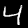
\includegraphics{images/mnist_2.png}\,
    
\includegraphics{images/mnist_3.png}\,
    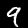
\includegraphics{images/mnist_4.png}
    }
    \end{center}
    Each $28\times28$ pixel image depicts a handwritten digit.  The training set
    consists of 60,000 examples, and the test set of 10,000 examples.  The task
    is, of course, to classify each image as a digit 0--9.
    \end{example}

    A large portion of the algorithms that have been successful at a range of
    tasks are in some sense `only a step or two away from linear'.  For
    instance, a basic approach to binary classification is to try to separate
    the points in the two classes by some hyperplane.  The Support Vector
    Machine is a modification of this approach that transforms the data to some
    even-higher dimensional space, and separates by a hyperplane there.  Another
    common approach is to consider linear combinations of some family of basis
    functions.

    For some problems, however, these techniques may not be enough.  Within the
    past ten years, this has prompted the creation of so-called `deep learning'
    methods.  An overview of the motivating problems of deep learning is
    contained in \cite{Ben09}.  Perhaps the most influential technique put forward so far is the
    Deep Belief Network.

\section{The Deep Belief Network}
    A Deep Belief Network (DBN) is a generative model consisting essentially a
    stack of RBMs, trained greedily.  The paper \cite{Hin07} introduced a
    technique known as `contrastive divergence' that allowed RBMs, and in turn
    DBNs, to be trained efficiently on problems of practical interest.
    \begin{definition}
    A \emph{Deep Belief Network} is a model on multiple layers of hidden
    variables, built out of RBMs.  Specifically, let $h^k \in \{0,1\}^{n_k}$
    denote the binary state vector of the $k^{\text{th}}$ layer for $0 \le k \le
    m$.  The layer $h^0$ is the visible layer.  The joint distribution of the
    DBN is
    \begin{align*}
        P(v,h^1, \ldots, h^m) &= P(h^{m-1}, h^m) \prod_{k=0}^{m-2} P(h^k \mid h^{k+1})\\
        P(h^k\mid h^{k+1}) &\propto \exp\pdil*{(h^k)^Tb^k + (h^k)^T W^{k+1} h^{k+1}}\\
        P(h^{m-1}, h^{m}) &\propto  \exp\pdil*{(h^{m-1})^T b^k + (h^{m-1})^T W^m
        h^m + (h^m)^T b^m}
    \end{align*}
    for some collection of parameters $b^k$ and $W^k$.
    \end{definition}

    The conditional independence structure of the DBN is described by a graph
    with undirected connections between the top two layers and directed
    connections between all other adjacent layers.
    \begin{center}
    \scalebox{0.6}{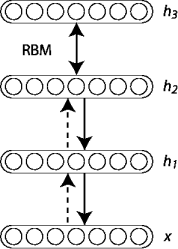
\includegraphics{images/DBN3.png}}
    \end{center}
    For classification, the network would be greedily trained to represent the
    input data.  The top layer $h^m$ would then be trained to classify the
    inputs with a one-hot encoding.

\appendix

\section{Affine and Projective Algebraic Geometry}

    The field of algebraic geometry grew out of the study of curves and surfaces
    determined by polynomials.  Beginning in the \oldstylenums{1950}s, the
    foundations of the subject were reforumlated by Serre and Grothendieck using
    sheaves and schemes.  More recently, the branch of computational algebraic
    geometry \ldots Gröbner bases.

    A standard introduction to algebraic geometry from a computational
    perspective is \cite{CLO92}, which is at a relatively elementary level.  The
    same authors have a graduate text \cite{CLO98}.

    Here, we introduce some classical objects.


\subsection{Affine and Projective Varieties}
    Throughout, let $\F$ be a field.  It is useful to think of $\F$ being either
    $\R$ or $\C$.

    Let $\A^n$ be the affine space of dimension $n$ over $\F$.  A polynomial $f
    \in \F[x_1, \ldots, x_n]$ can be considered as a function on $\A^n$ by
    simply evaluating the polynomial on any given point.

    \begin{definition}
        An \emph{affine variety} is any subset of the affine space $\A^n$ of the
        form
        \[
            V(f_1, \ldots, f_m)
            = \cdil[\big]{x \in \A^n \vbar f_i(x) = 0 \quad\text{for all $i$}}
        \]
        for some finite set of polynomials $f_i \in \F[x_1, \ldots, x_n]$.
    \end{definition}
    \noindent (Note that some authors instead use the term `affine algebraic
    set' and reserve `affine variety' for irreducible sets.) Instead of a finite
    set of polynomials, we can equivalently consider a finitely generated ideal.
    In fact, $\F[x_1,\ldots,x_n]$ is a Noetherian ring, so the condition that
    the ideal be finitely generated condition is redundant.

    Given a subset $X \subset \A^n$, we may consider the ideal of polynomials
    vanishing on the subset
    \[
        I(X) = \cdil[\big]{f \in \F[x_1, \ldots, x_n] \vbar f(x) = 0 \quad\text{for
        all $x \in X$}}.
    \]
    Under certain conditions (which depend on the field $\F$), the operations
    $V$ and $I$ are inverses of each other.

    \begin{definition}
        The \emph{projective space} of dimension $n$ (usually denoted $\Proj^n$)
        is the space $\F^{n+1}\setminus \{0\}$ under the equivalence relation $x
        \sim \lambda x$ for $x \in \F^{n+1}$ and $0 \ne \lambda \in \F$.  The
        usual affine coordinates on $\F^{n+1}$ give \emph{homogeneous
        coordinates} $[x_0: \cdots: x_n]$ on $\Proj^n$.  If $\F = \R$ (resp.
        $\C$), the homogeneous coordinates can be used to construct coordinate
        charts, giving $\Proj^n$ the structure of a real (resp. complex)
        manifold.
    \end{definition}

    Projective space may also be thought of as the inductively-defined space
    \[
        \Proj^0 = \{\ast\}, \qquad \Proj^n = \A^n \cup \Proj^{n-1}.
    \]
    It also turns out that projective space behaves particularly nicely for the
    purposes of algebraic geometry, for reasons that we will not describe here.
    Instead of arbitrary polynomials, a different collection of `functions' is
    used on projective space.
    \begin{definition}
        A \emph{homogeneous polynomial} in $n+1$ variables of degree $d$ is a
        polynomial of the form $F(x) = \sum a_I x^I$ where $a_I \in \F$ and the
        multi-index ranges over $I = (i_0, \ldots, i_n)$ such that $i_0 + \cdots
        + i_n = d$.  The monomials are defined to be $x^I = x_0^{i_0}\cdots
        x_n^{i_n}$.  A \emph{homogeneous ideal} is an ideal of $\F[x_0, \ldots,
        x_n]$ generated by homogeneous polynomials.
    \end{definition}
    Notice that if $F$ is homogeneous polynomial of degree $d$, then $F(\lambda
    x) = \lambda^d F(x)$ for $\lambda \in \F$.  The zero set of $F$ in $\Proj^n$
    is then well-defined.  It follows that we can define a projective analogue
    of an affine variety.
    \begin{definition}
        A \emph{projective variety} is any subset of the projective space
        $\Proj^n$ of the form
        \[
            V(f_1, \ldots, f_m)
            = \cdil[\big]{x \in \Proj^n \vbar f_i(x) = 0 \quad\text{for all $i$}}
        \]
        for some finite set of homogeneous polynomials $f_i \in \F[x_0,
        \ldots,x_n]$.
    \end{definition}
    As in the affine case, there is a well-behaved correspondence between the
    homogeneous ideals of $\F[x_0, \ldots, x_n]$ and projective varieties.

    Using these varieties, we may define the \emph{Zariski topology} on $\A^n$
    and $\Proj^n$;  the affine (or projective) varieties are the closed sets of
    the topology.  It is straightforward to show that the Zariski topology is,
    in fact, a topology.

    For the applications encountered in algebraic statistics, we will need to
    venture into real algebraic geometry, the primary objects of which are
    slightly less well-behaved.
    \begin{definition}
        A \emph{semialgebraic set} is any subset of $\R^n$ of the form
        \[
            V = \cdil[\big]{ x \in \R^n \vbar
                f_i(x) = 0, g_j(x) > 0
            \quad\text{for all $i,j$}}
        \]
        for some finite collection of polynomials $f_i, g_j \in \R[x_1, \ldots,
        x_n]$.
    \end{definition}

    A more in-depth investigation into algebraic geometry reveals the central
    importance of rings of functions on spaces, and the need to consider
    arbitrary commutative rings.  This road leads to the theory of schemes,
    which we will neither need nor pursue here.

\section{A Primer on Machine Learning}

\nocite{*}
\bibliographystyle{annotate}
\bibliography{mid}

\begin{comment}
\begin{thebibliography}{100}
    \bibitem[BCR98]{BCR98} Bochnak, Coste, Roy.  Real Algebraic Geometry.  1998.
    \bibitem[Ben09]{Ben09} Bengio.  Learning Deep Architectures for AI. 2009.
    \bibitem[CLO92]{CLO92} Cox, Little, O'Shea.  Ideals, Varieties, and
    Algorithms.  1992.
    \bibitem[CLO98]{CLO98} Cox, Little, O'Shea.  Using Algebraic Geometry.  1998.
    \bibitem[CLS09]{CLS09} Cox, Little, Schenck.  Toric Varieties.  2009.
    \bibitem[CMS09]{CMS09} Cueto, Morton, Sturmfels. Geometry of the Restricted Boltzmann Machine.  2009.
    \bibitem[Cos09]{Cos09} Michel Coste.  An Introduction to Semialgebraic Geometry.  2002.
    \bibitem[CTY10]{CTY10} Cueto, Tobis, Yu.  An Implicitization Challenge for Binary Factor Analysis. 
    2010.
    \bibitem[DS98]{DS98} Diaconis and Sturmfels.  Algebraic Algorithms for Sampling
    from Conditional Distributions. 1998.
    \bibitem[DSS09]{DSS09} Drton, Sturmfels, Sullivant. Lectures on Algebraic
    Statistics. 2009.
    \bibitem[GMS06]{GMS06} Geiger, Meed, Sturmfels.  On the Toric Algebra of Graphical Models. 2006.
    \bibitem[Hin07]{Hin07} Hinton.  A Fast Algorithm for Deep Belief Nets.  2007.
    \bibitem[MA10]{MA10} Montufar, Ay.  Refinements of Universal Approximation
    Results for Deep Belief Networks and Restricted Boltzmann Machines.  2010.
    \bibitem[Mon10]{Mon10} Montufar.  Mixture Models and Representational Power of
    RBM's, DBN's and DBM's.  2010.
    \bibitem[PS03]{PS03} Pachter, Sturmfels.  Tropical Geometry of Statistical Models. 2003.
    \bibitem[Ric09]{Ric09} Riccomagno.  A Short History of Algebraic Statistics.  2009.
    \bibitem[Top02]{Top02} Topics in Algebraic Geometry and Geometric Modeling:
    Workshop on Algebraic Geometry and Geometric Modeling July 29 -- August 2,
    2002 (Contemporary Mathematics).  Ed. by Goldman and Krasauskas.
    \bibitem[Wat09]{Wat09} Watanabe.  Algebraic Geometry and Statistical Learning Theory.  2009.

    \bibitem{A5} Pachter, Sturmfels.  ``Tropical Geometry of Statistical
    Models''. 2003.
    \bibitem{A6} Pachter, Sturmfels.  \textit{Algebraic Statistics for
    Computational Biology}.  2005.
\end{thebibliography}
\end{comment}


\end{document}
